\documentclass[english, 11pt]{article}\usepackage[]{graphicx}\usepackage[]{color}
%% maxwidth is the original width if it is less than linewidth
%% otherwise use linewidth (to make sure the graphics do not exceed the margin)
\makeatletter
\def\maxwidth{ %
  \ifdim\Gin@nat@width>\linewidth
    \linewidth
  \else
    \Gin@nat@width
  \fi
}
\makeatother

\definecolor{fgcolor}{rgb}{0.345, 0.345, 0.345}
\newcommand{\hlnum}[1]{\textcolor[rgb]{0.686,0.059,0.569}{#1}}%
\newcommand{\hlstr}[1]{\textcolor[rgb]{0.192,0.494,0.8}{#1}}%
\newcommand{\hlcom}[1]{\textcolor[rgb]{0.678,0.584,0.686}{\textit{#1}}}%
\newcommand{\hlopt}[1]{\textcolor[rgb]{0,0,0}{#1}}%
\newcommand{\hlstd}[1]{\textcolor[rgb]{0.345,0.345,0.345}{#1}}%
\newcommand{\hlkwa}[1]{\textcolor[rgb]{0.161,0.373,0.58}{\textbf{#1}}}%
\newcommand{\hlkwb}[1]{\textcolor[rgb]{0.69,0.353,0.396}{#1}}%
\newcommand{\hlkwc}[1]{\textcolor[rgb]{0.333,0.667,0.333}{#1}}%
\newcommand{\hlkwd}[1]{\textcolor[rgb]{0.737,0.353,0.396}{\textbf{#1}}}%
\let\hlipl\hlkwb

\usepackage{framed}
\makeatletter
\newenvironment{kframe}{%
 \def\at@end@of@kframe{}%
 \ifinner\ifhmode%
  \def\at@end@of@kframe{\end{minipage}}%
  \begin{minipage}{\columnwidth}%
 \fi\fi%
 \def\FrameCommand##1{\hskip\@totalleftmargin \hskip-\fboxsep
 \colorbox{shadecolor}{##1}\hskip-\fboxsep
     % There is no \\@totalrightmargin, so:
     \hskip-\linewidth \hskip-\@totalleftmargin \hskip\columnwidth}%
 \MakeFramed {\advance\hsize-\width
   \@totalleftmargin\z@ \linewidth\hsize
   \@setminipage}}%
 {\par\unskip\endMakeFramed%
 \at@end@of@kframe}
\makeatother

\definecolor{shadecolor}{rgb}{.97, .97, .97}
\definecolor{messagecolor}{rgb}{0, 0, 0}
\definecolor{warningcolor}{rgb}{1, 0, 1}
\definecolor{errorcolor}{rgb}{1, 0, 0}
\newenvironment{knitrout}{}{} % an empty environment to be redefined in TeX

\usepackage{alltt}
\usepackage[utf8]{inputenc}
\usepackage{booktabs}
\usepackage{booktabs}
\usepackage{longtable}
\usepackage{array}
\usepackage{multirow}
\usepackage[table]{xcolor}
\usepackage{wrapfig}
\usepackage{float}
\usepackage{colortbl}
\usepackage{pdflscape}
\usepackage{tabu}
\usepackage{threeparttable}
\usepackage[normalem]{ulem}
\IfFileExists{upquote.sty}{\usepackage{upquote}}{}
\begin{document}


\title{Problem Set 1}
\author{Sébastien Annan-Phan, Alejandro Favela, Matthew Tadruno }

\maketitle






\newpage
\noindent \section*{Questions 1 and 2} Reading and cleaning the data.
\begin{knitrout}\small
\definecolor{shadecolor}{rgb}{0.969, 0.969, 0.969}\color{fgcolor}\begin{kframe}
\begin{alltt}
\hlstd{wb_data} \hlkwb{<-}\hlkwd{read_csv}\hlstd{(}\hlkwd{paste0}\hlstd{(dir_data,} \hlstr{"ps1_raw.csv"}\hlstd{),} \hlkwc{col_types}\hlstd{=}\hlkwd{cols}\hlstd{())}

\hlcom{#Assigning column names }
\hlkwd{colnames}\hlstd{(wb_data)} \hlkwb{<-}
  \hlkwd{c}\hlstd{(}\hlstr{"year"}\hlstd{,} \hlstr{"year_code"}\hlstd{,} \hlstr{"country"}\hlstd{,}
    \hlstr{"country_code"}\hlstd{,} \hlstr{"CO2"}\hlstd{,} \hlstr{"GDP"}\hlstd{,} \hlstr{"POP"}\hlstd{)}

\hlcom{#dropping year code }
\hlstd{wb_data} \hlkwb{<-} \hlkwd{select}\hlstd{(wb_data,} \hlopt{-}\hlstd{year_code)}

\hlcom{#drop ".." observations}
\hlstd{vars}\hlkwb{<-}\hlkwd{names}\hlstd{(wb_data)[}\hlnum{4}\hlopt{:}\hlnum{6}\hlstd{]}
\hlkwa{for} \hlstd{(var} \hlkwa{in} \hlstd{vars) \{}
  \hlstd{wb_data} \hlkwb{<-} \hlstd{wb_data[}\hlopt{!}\hlstd{wb_data[var]} \hlopt{==} \hlstr{".."}\hlstd{, ]}
\hlstd{\}}

\hlstd{wb_data} \hlkwb{<-} \hlkwd{na.omit}\hlstd{(wb_data)}
\hlstd{wb_data[}\hlnum{4}\hlopt{:}\hlnum{6}\hlstd{]} \hlkwb{<-}\hlkwd{lapply}\hlstd{(wb_data[}\hlnum{4}\hlopt{:}\hlnum{6}\hlstd{], as.numeric)}
\end{alltt}
\end{kframe}
\end{knitrout}

\noindent \section*{Question 3} Calculate a table of showing the sample mean, standard deviation, minimum and maximum for each series.



\begin{knitrout}
\definecolor{shadecolor}{rgb}{0.969, 0.969, 0.969}\color{fgcolor}\begin{table}[!h]

\caption{\label{tab:Q.3 output}Summary Statistics}
\centering
\begin{tabular}[t]{lrrr}
\toprule
  & CO\textsubscript{2} (kt) & GDP (2010 USD) & Population\\
\midrule
Mean & 162316.561 & 3.363660e+11 & 35220247\\
S.D. & 763012.353 & 1.297364e+12 & 134642965\\
Min & 7.334 & 3.182352e+07 & 10025\\
Max & 8776040.416 & 1.496437e+13 & 1337705000\\
\bottomrule
\end{tabular}
\end{table}


\end{knitrout}



\newpage
\bigskip
\noindent \section*{Question 4} Create a histogram for CO\textsubscript{2} and GDP (15 buckets).
\vspace{2mm}

\begin{knitrout}
\definecolor{shadecolor}{rgb}{0.969, 0.969, 0.969}\color{fgcolor}
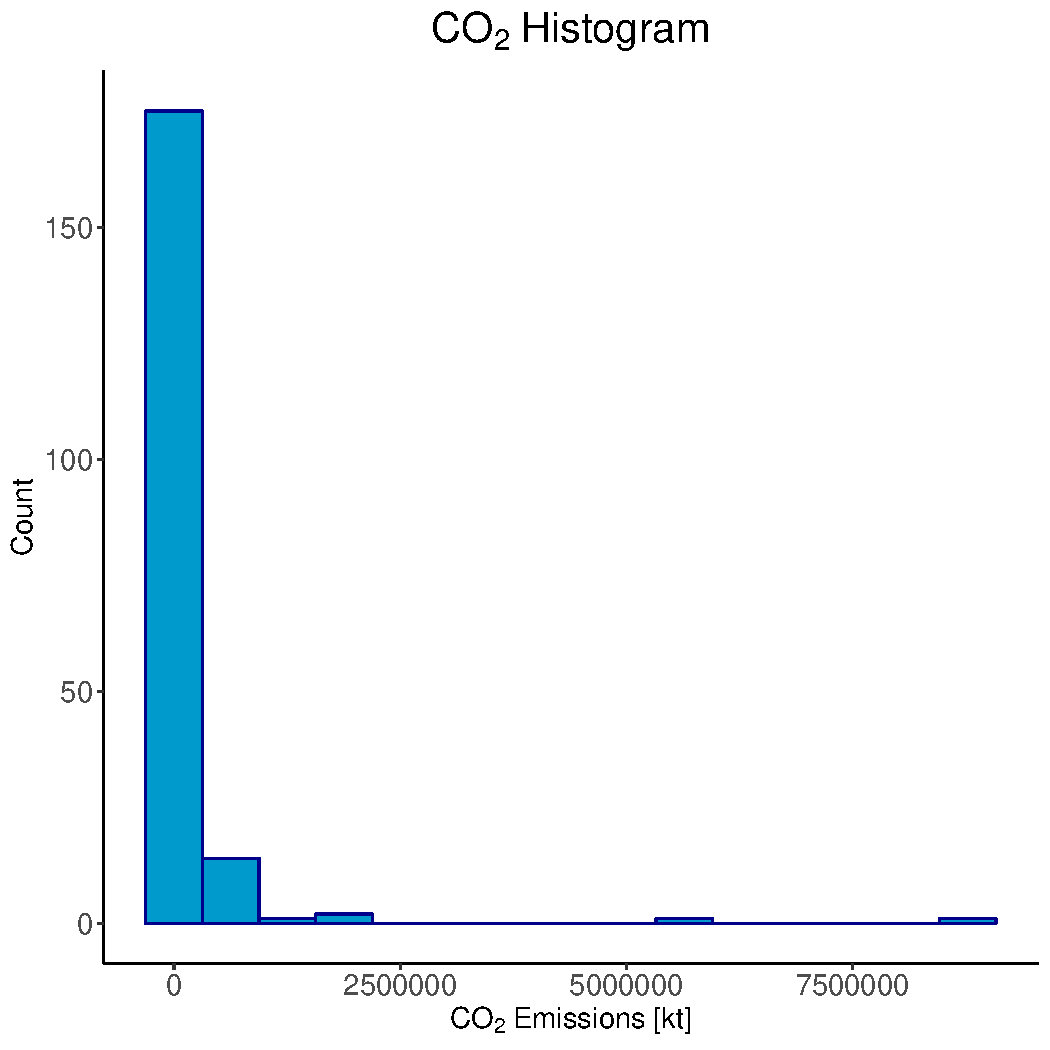
\includegraphics[width=7cm,height=7cm]{figure/Q_4_output-1} 
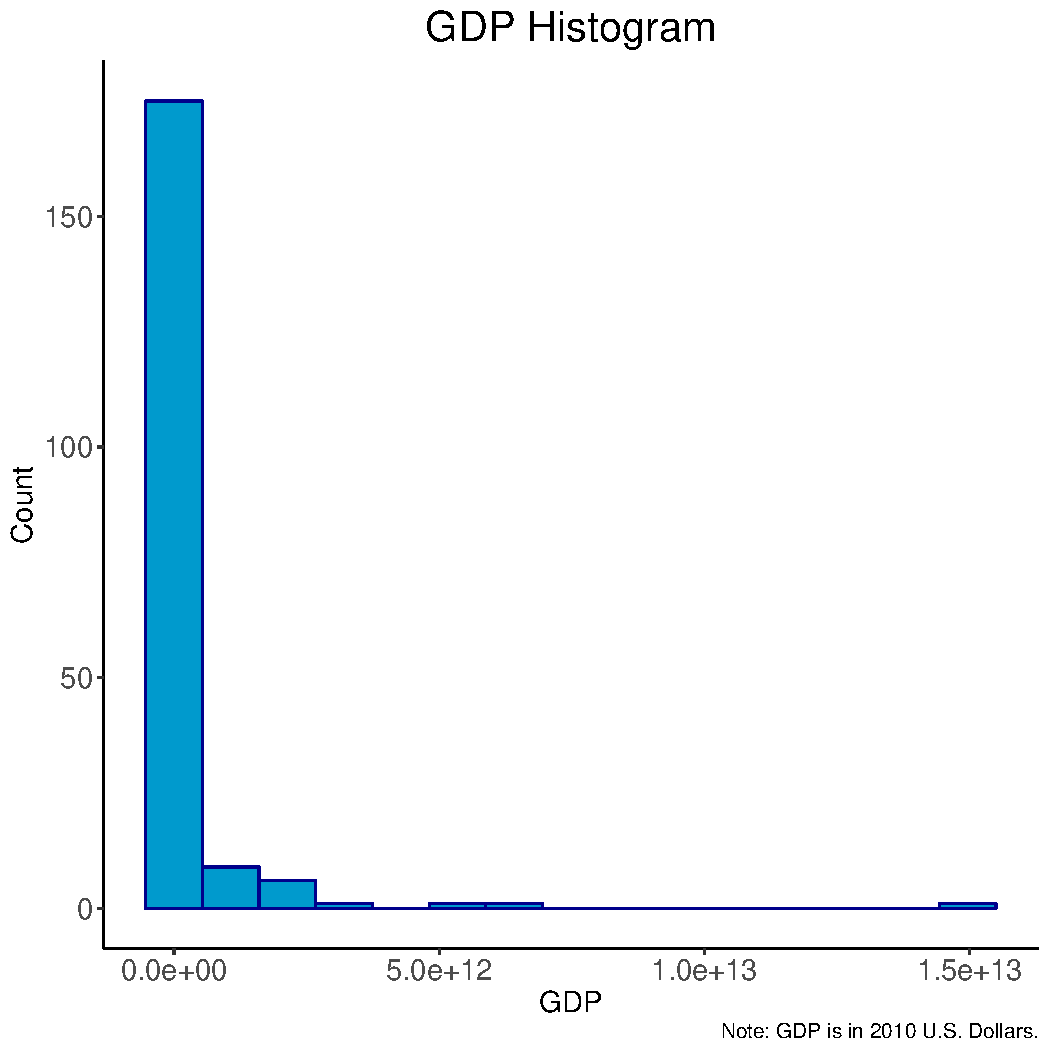
\includegraphics[width=7cm,height=7cm]{figure/Q_4_output-2} 

\end{knitrout}


\noindent \section*{Question 5} Plot CO\textsubscript{2} against GDP. 
\vspace{2mm}

\begin{knitrout}
\definecolor{shadecolor}{rgb}{0.969, 0.969, 0.969}\color{fgcolor}

{\centering 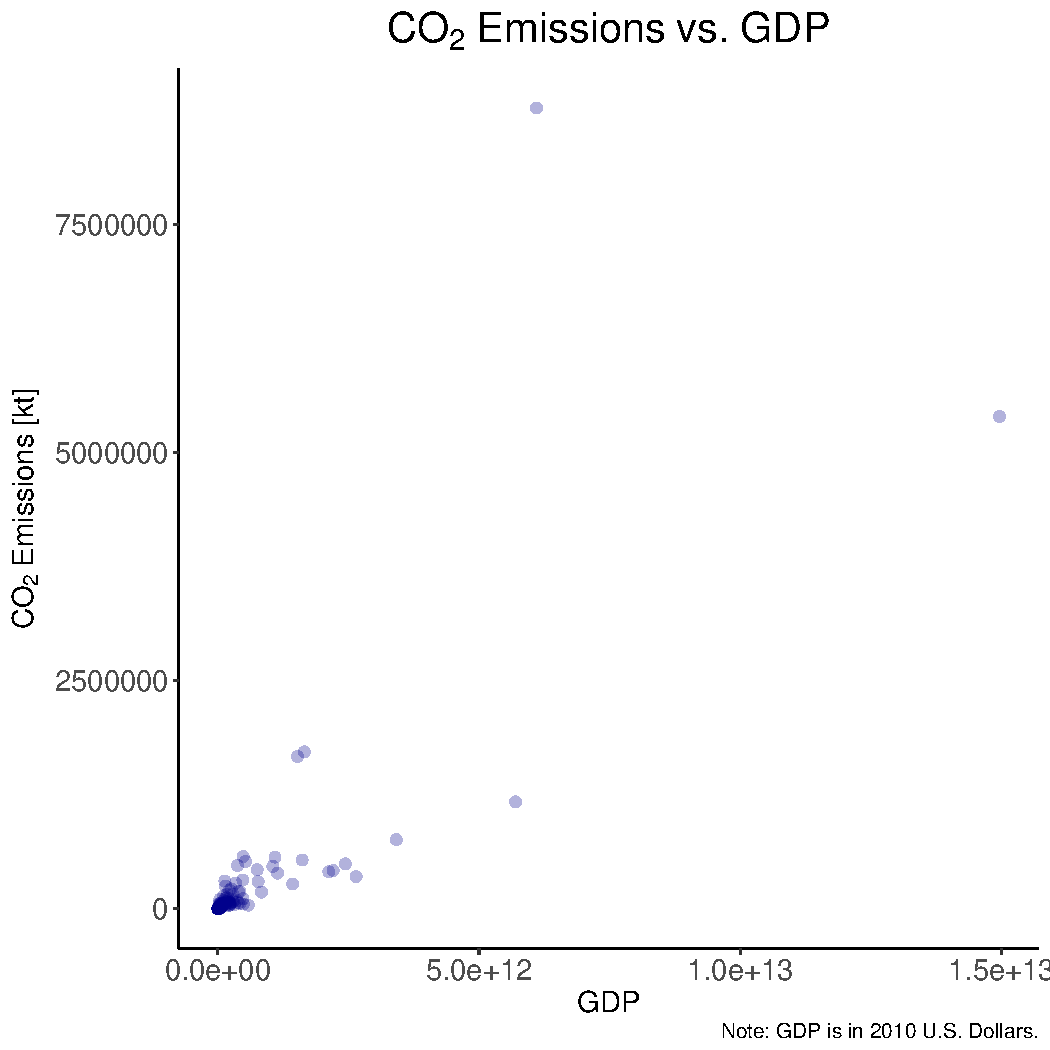
\includegraphics[width=8cm,height=8cm]{figure/Q_5_graph_output-1} 

}



\end{knitrout}

\noindent \section*{Question 6} Create a new variable “Per capita CO\textsubscript{2} emissions” called \textit{CO2pc}.
\begin{knitrout}
\definecolor{shadecolor}{rgb}{0.969, 0.969, 0.969}\color{fgcolor}\begin{kframe}
\begin{alltt}
\hlstd{wb_data}\hlopt{$}\hlstd{CO2pc}\hlkwb{<-}\hlstd{wb_data}\hlopt{$}\hlstd{CO2}\hlopt{/}\hlstd{wb_data}\hlopt{$}\hlstd{POP}
\end{alltt}
\end{kframe}
\end{knitrout}

\noindent \section*{Question 7} Create a new variable “Per capita GDP” called \textit{GDPpc}.
\begin{knitrout}
\definecolor{shadecolor}{rgb}{0.969, 0.969, 0.969}\color{fgcolor}\begin{kframe}
\begin{alltt}
\hlstd{wb_data}\hlopt{$}\hlstd{GDPpc}\hlkwb{<-}\hlstd{wb_data}\hlopt{$}\hlstd{GDP}\hlopt{/}\hlstd{wb_data}\hlopt{$}\hlstd{POP}
\end{alltt}
\end{kframe}
\end{knitrout}
  
\noindent \section*{Question 8} Plot \textit{CO2pc} against \textit{GDPpc}.
\vspace{5mm}

\begin{knitrout}
\definecolor{shadecolor}{rgb}{0.969, 0.969, 0.969}\color{fgcolor}

{\centering 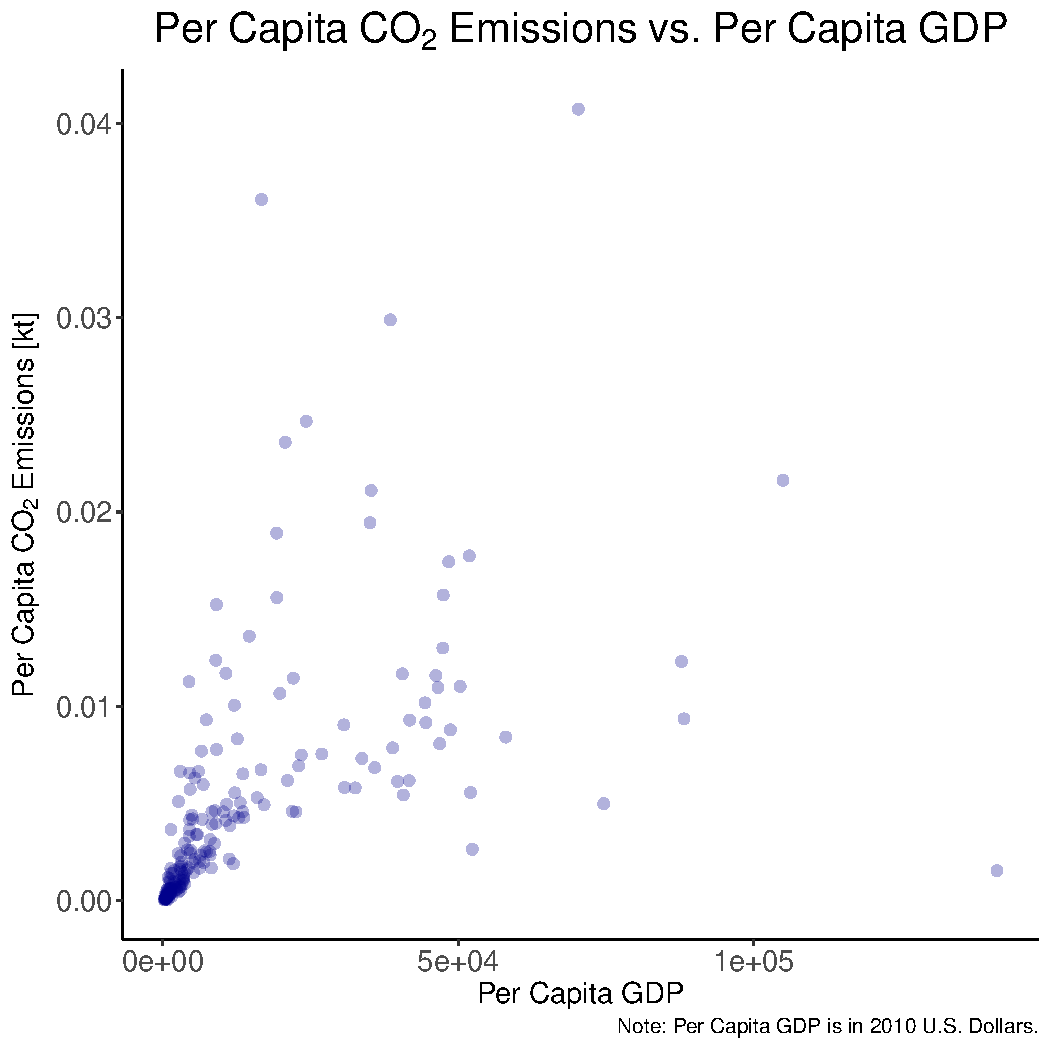
\includegraphics[width=8cm,height=8cm]{figure/Q_8_output-1} 

}



\end{knitrout}

\newpage
\noindent \section*{Question 9}  Create demeaned variables of \textit{CO2pc} and \textit{GDPpc} called \textit{CO2pcdev} and \textit{GDPpcdev} by subtracting the sample mean from each observation.
\begin{knitrout}
\definecolor{shadecolor}{rgb}{0.969, 0.969, 0.969}\color{fgcolor}\begin{kframe}
\begin{alltt}
\hlstd{wb_data}\hlopt{$}\hlstd{CO2pcdev}\hlkwb{<-}\hlstd{wb_data}\hlopt{$}\hlstd{CO2pc}\hlopt{-}\hlkwd{mean}\hlstd{(wb_data}\hlopt{$}\hlstd{CO2pc)}
\hlstd{wb_data}\hlopt{$}\hlstd{GDPpcdev}\hlkwb{<-}\hlstd{wb_data}\hlopt{$}\hlstd{GDPpc}\hlopt{-}\hlkwd{mean}\hlstd{(wb_data}\hlopt{$}\hlstd{GDPpc)}
\end{alltt}
\end{kframe}
\end{knitrout}

\bigskip
\noindent \section*{Question 10} Plot \textit{CO2pcdev} against \textit{GDPpcdev}.
\vspace{5mm}

\begin{knitrout}
\definecolor{shadecolor}{rgb}{0.969, 0.969, 0.969}\color{fgcolor}

{\centering 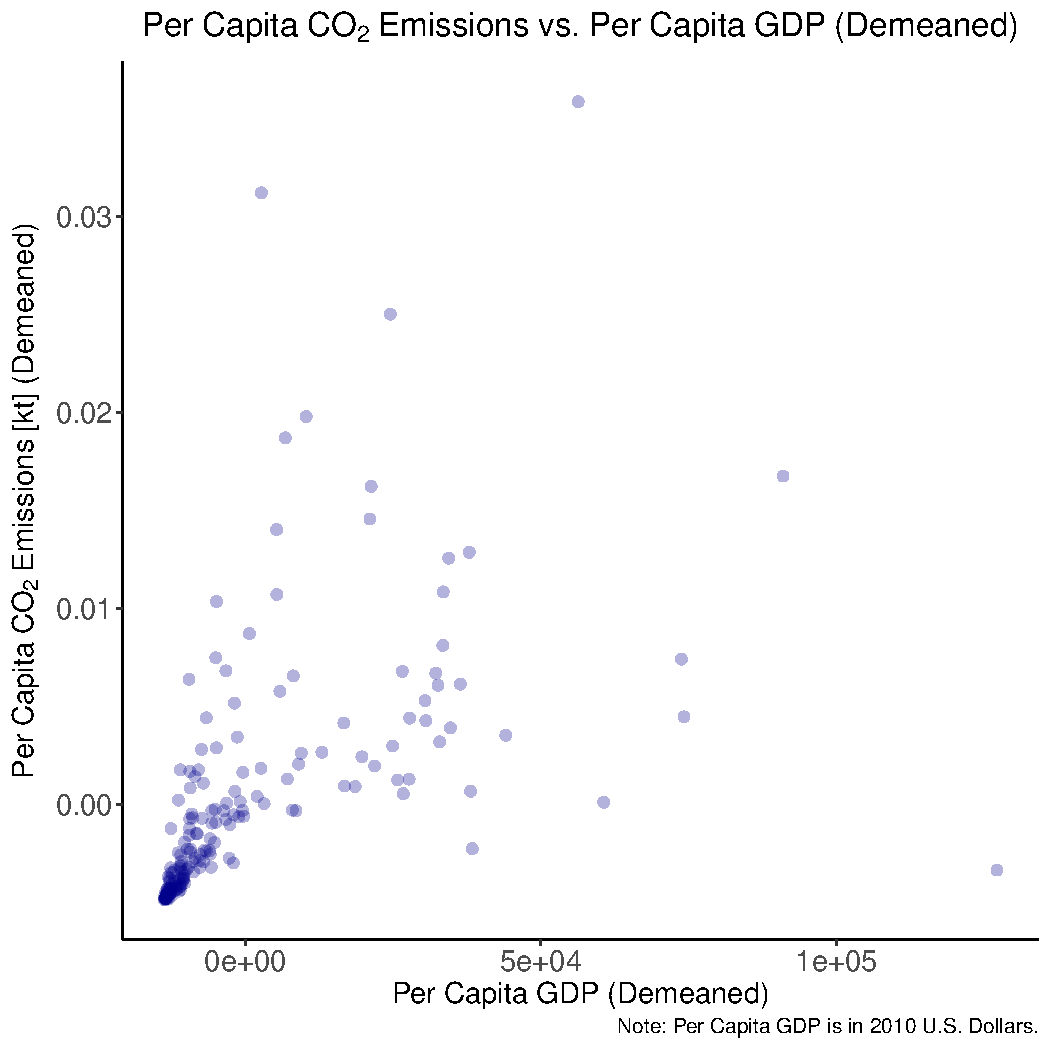
\includegraphics[width=8cm,height=8cm]{figure/Q_10_output-1} 

}



\end{knitrout}

\noindent \section*{Question 11} Create the variables \textit{CO2pcln} and \textit{GDPpcln} by taking natural logs of \textit{CO2pc} and \textit{GDPpc}.
\vspace{5mm}
\begin{knitrout}
\definecolor{shadecolor}{rgb}{0.969, 0.969, 0.969}\color{fgcolor}\begin{kframe}
\begin{alltt}
\hlstd{wb_data}\hlopt{$}\hlstd{CO2pcln}\hlkwb{<-}\hlkwd{log}\hlstd{(wb_data}\hlopt{$}\hlstd{CO2pc)}
\hlstd{wb_data}\hlopt{$}\hlstd{GDPpcln}\hlkwb{<-}\hlkwd{log}\hlstd{(wb_data}\hlopt{$}\hlstd{GDPpc)}
\end{alltt}
\end{kframe}
\end{knitrout}

\bigskip
\noindent \section*{Question 12} Plot \textit{CO2pcln} and \textit{GDPpcln}.
\vspace{5mm}

\begin{knitrout}
\definecolor{shadecolor}{rgb}{0.969, 0.969, 0.969}\color{fgcolor}

{\centering 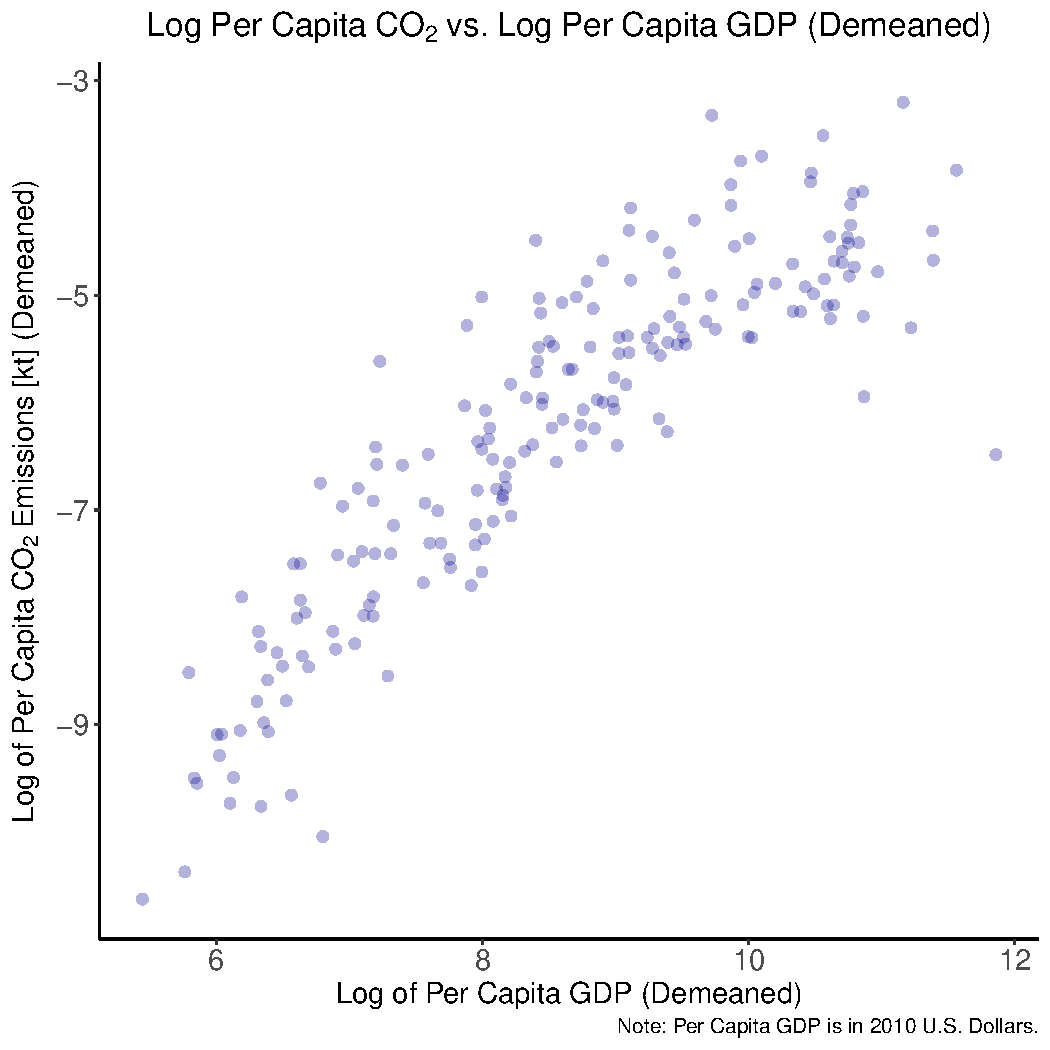
\includegraphics[width=8cm,height=8cm]{figure/Q_12_output-1} 

}



\end{knitrout}

\noindent \section*{Question 13} Export your data as a comma delimited ascii file.
\begin{knitrout}
\definecolor{shadecolor}{rgb}{0.969, 0.969, 0.969}\color{fgcolor}\begin{kframe}
\begin{alltt}
\hlkwd{write.csv}\hlstd{(wb_data,} \hlkwc{file} \hlstd{=} \hlstr{"wb_formatted.csv"}\hlstd{)}
\hlcom{#default ascii}
\end{alltt}
\end{kframe}
\end{knitrout}

\newpage
\noindent \section*{Custom OLS Function} 
\begin{knitrout}\footnotesize
\definecolor{shadecolor}{rgb}{0.969, 0.969, 0.969}\color{fgcolor}\begin{kframe}
\begin{alltt}
\hlstd{b_ols} \hlkwb{<-} \hlkwa{function}\hlstd{(}\hlkwc{data}\hlstd{,} \hlkwc{y}\hlstd{,} \hlkwc{X}\hlstd{,} \hlkwc{intercept}\hlstd{=}\hlkwa{NULL}\hlstd{) \{}
  \hlcom{# This function takes as inputs:}
  \hlcom{# 1. A data frame, 'data'}
  \hlcom{# 2. A dependent variable, y }
  \hlcom{# 3. A list of X variables c("x1", "x2", ...)}
  \hlcom{# 4. An optional 4th argument, T, to include an intercept }
  \hlkwd{require}\hlstd{(dplyr)}

  \hlcom{# Select y variable data from 'data'}
  \hlstd{y_data} \hlkwb{<-} \hlkwd{subset}\hlstd{(data,} \hlkwc{select}\hlstd{=}\hlkwd{c}\hlstd{(y))}
  \hlcom{# Select X variable data from 'data'}
  \hlstd{X_data} \hlkwb{<-} \hlkwd{select_}\hlstd{(data,} \hlkwc{.dots} \hlstd{= X)}

  \hlkwa{if}\hlstd{(}\hlkwd{is.null}\hlstd{(intercept)) \{}
    \hlcom{# Convert y_data to matrices}
    \hlstd{y_data} \hlkwb{<-} \hlkwd{as.matrix}\hlstd{(y_data)}
    \hlcom{# Convert X_data to matrices}
    \hlstd{X_data} \hlkwb{<-} \hlkwd{as.matrix}\hlstd{(X_data)}
    \hlcom{# Calculate beta hat}
    \hlstd{beta_hat} \hlkwb{<-} \hlkwd{solve}\hlstd{(}\hlkwd{t}\hlstd{(X_data)}\hlopt\hlstd{X_data)}\hlopt\hlkwd{t}\hlstd{(X_data)}\hlopt\hlstd{y_data}
  \hlstd{\}}

  \hlkwa{else}\hlstd{\{}
    \hlcom{# Convert y_data to matrices}
    \hlstd{y_data} \hlkwb{<-} \hlkwd{as.matrix}\hlstd{(y_data)}
    \hlcom{# Add a column of ones to X_data }
    \hlstd{X_data} \hlkwb{<-} \hlkwd{mutate_}\hlstd{(X_data,} \hlstr{"ones"} \hlstd{=} \hlnum{1}\hlstd{)}
    \hlcom{# Move the intercept column to the front (this is cool)}
    \hlstd{X_data} \hlkwb{<-} \hlkwd{select_}\hlstd{(X_data,} \hlstr{"ones"}\hlstd{,} \hlkwc{.dots} \hlstd{= X)}
    \hlcom{# Convert X_data to matrices}
    \hlstd{X_data} \hlkwb{<-} \hlkwd{as.matrix}\hlstd{(X_data)}
    \hlcom{# Calculate beta hat}
    \hlstd{beta_hat} \hlkwb{<-} \hlkwd{solve}\hlstd{(}\hlkwd{t}\hlstd{(X_data)}\hlopt\hlstd{X_data)}\hlopt\hlkwd{t}\hlstd{(X_data)}\hlopt\hlstd{y_data}
    \hlcom{# Change the name of 'ones' to 'intercept'}
    \hlkwd{rownames}\hlstd{(beta_hat)} \hlkwb{<-} \hlkwd{c}\hlstd{(}\hlstr{"intercept"}\hlstd{, X)}
  \hlstd{\}}

  \hlstd{y_hat}\hlkwb{<-}\hlstd{X_data}\hlopt\hlstd{beta_hat} \hlcom{#Predicted values}
  \hlstd{residual}\hlkwb{<-}\hlstd{y_data} \hlopt{-} \hlstd{y_hat}

  \hlstd{SST}\hlkwb{<-}\hlkwd{sum}\hlstd{((y_data)}\hlopt{^}\hlnum{2}\hlstd{)} \hlcom{#Total sum of squares }
  \hlstd{SSM}\hlkwb{<-}\hlkwd{sum}\hlstd{((y_hat)}\hlopt{^}\hlnum{2}\hlstd{)} \hlcom{#Regression sum of squares}
  \hlstd{SSR}\hlkwb{<-}\hlkwd{sum}\hlstd{((y_data}\hlopt{-}\hlstd{y_hat)}\hlopt{^}\hlnum{2}\hlstd{)} \hlcom{#Error sum of squares}

  \hlstd{SSM_demean} \hlkwb{<-} \hlkwd{sum}\hlstd{((y_hat} \hlopt{-} \hlkwd{mean}\hlstd{(y_data))}\hlopt{^}\hlnum{2}\hlstd{)}
  \hlstd{SST_demean} \hlkwb{<-} \hlkwd{sum}\hlstd{((y_data} \hlopt{-} \hlkwd{mean}\hlstd{(y_data))}\hlopt{^}\hlnum{2}\hlstd{)}

  \hlstd{n} \hlkwb{<-} \hlkwd{dim}\hlstd{(X_data)[}\hlnum{1}\hlstd{]}
  \hlstd{k} \hlkwb{<-} \hlkwd{dim}\hlstd{(X_data)[}\hlnum{2}\hlstd{]}
  \hlstd{dof} \hlkwb{<-} \hlstd{n} \hlopt{-} \hlstd{k}
  \hlstd{R_uc} \hlkwb{<-} \hlnum{1} \hlopt{-} \hlstd{(SSR}\hlopt{/}\hlstd{SST)}
  \hlstd{R} \hlkwb{<-} \hlnum{1}\hlopt{-} \hlstd{SSR}\hlopt{/}\hlstd{SST_demean}
  \hlstd{R_adj} \hlkwb{<-} \hlnum{1} \hlopt{-} \hlstd{(}\hlnum{1} \hlopt{-} \hlstd{R)} \hlopt{*} \hlstd{((n}\hlopt{-}\hlnum{1}\hlstd{)}\hlopt{/}\hlstd{(n}\hlopt{-}\hlstd{k))}
  \hlstd{AIC} \hlkwb{<-} \hlkwd{log}\hlstd{(SSR}\hlopt{/}\hlstd{n)} \hlopt{+} \hlstd{(}\hlnum{2}\hlopt{*}\hlstd{k)}\hlopt{/}\hlstd{n}
  \hlstd{SIC} \hlkwb{<-} \hlkwd{log}\hlstd{(SSR}\hlopt{/}\hlstd{n)} \hlopt{+} \hlstd{(k}\hlopt{/}\hlstd{n)} \hlopt{*} \hlkwd{log}\hlstd{(n)}
  \hlstd{s2} \hlkwb{<-} \hlstd{SSR}\hlopt{/}\hlstd{(n}\hlopt{-}\hlstd{k)}

  \hlkwd{assign}\hlstd{(}\hlstr{"y_hat"}\hlstd{, y_hat, .GlobalEnv)}
  \hlkwd{assign}\hlstd{(}\hlstr{"residual"}\hlstd{, residual, .GlobalEnv)}
  \hlkwd{assign}\hlstd{(}\hlstr{"beta_hat"}\hlstd{, beta_hat, .GlobalEnv)}
  \hlkwd{assign}\hlstd{(}\hlstr{"R"}\hlstd{, R, .GlobalEnv)}
  \hlkwd{assign}\hlstd{(}\hlstr{"R_uc"}\hlstd{, R_uc, .GlobalEnv)}
  \hlkwd{assign}\hlstd{(}\hlstr{"R_adj"}\hlstd{, R_adj, .GlobalEnv)}
  \hlkwd{assign}\hlstd{(}\hlstr{"AIC"}\hlstd{, R_uc, .GlobalEnv)}
  \hlkwd{assign}\hlstd{(}\hlstr{"SIC"}\hlstd{, SIC, .GlobalEnv)}
  \hlkwd{assign}\hlstd{(}\hlstr{"s2"}\hlstd{, s2, .GlobalEnv)}
  \hlkwd{assign}\hlstd{(}\hlstr{"n"}\hlstd{, n, .GlobalEnv)}
  \hlkwd{assign}\hlstd{(}\hlstr{"dof"}\hlstd{, dof, .GlobalEnv)}


  \hlstd{fit}\hlkwb{<-}\hlkwd{data.frame}\hlstd{(n, dof,} \hlkwd{round}\hlstd{(R,} \hlnum{4}\hlstd{),} \hlkwd{round}\hlstd{(R_uc,} \hlnum{4}\hlstd{),}
       \hlkwd{round}\hlstd{(R_adj,} \hlnum{4}\hlstd{),} \hlkwd{round}\hlstd{(AIC,} \hlnum{4}\hlstd{),} \hlkwd{round}\hlstd{(SIC,} \hlnum{4}\hlstd{),} \hlkwd{round}\hlstd{(s2,} \hlnum{4}\hlstd{))}
  \hlkwd{assign}\hlstd{(}\hlstr{"fit"}\hlstd{, fit, .GlobalEnv)}


  \hlkwd{return}\hlstd{(}\hlkwd{c}\hlstd{(beta_hat, R, R_uc, R_adj, AIC, SIC, s2))}
\hlstd{\}}
\end{alltt}
\end{kframe}
\end{knitrout}

\newpage
\noindent \section*{Question 14} Regress \textit{CO2pc} on \textit{GDPpc} without an intercept...

\begin{knitrout}
\definecolor{shadecolor}{rgb}{0.969, 0.969, 0.969}\color{fgcolor}\begin{kframe}
\begin{alltt}
\hlcom{#Regress CO2pc on GDPpc without an intercept}
\hlkwd{b_ols}\hlstd{(}\hlkwc{data} \hlstd{= wb_data,} \hlkwc{y}\hlstd{=}\hlstr{"CO2pc"}\hlstd{,} \hlkwc{X}\hlstd{=}\hlkwd{c}\hlstd{(}\hlstr{"GDPpc"}\hlstd{))[}\hlnum{1}\hlstd{]}
\end{alltt}
\begin{verbatim}
## [1] 2.233062e-07
\end{verbatim}
\begin{alltt}
\hlcom{# Regress CO2pc*1000 on GDPpc without an intercept}
\hlstd{wb_data}\hlopt{$}\hlstd{CO2pc}\hlkwb{<-}\hlstd{wb_data}\hlopt{$}\hlstd{CO2pc}\hlopt{*}\hlnum{1000}
\hlkwd{b_ols}\hlstd{(}\hlkwc{data} \hlstd{= wb_data,} \hlkwc{y}\hlstd{=}\hlstr{"CO2pc"}\hlstd{,} \hlkwc{X}\hlstd{=}\hlkwd{c}\hlstd{(}\hlstr{"GDPpc"}\hlstd{))[}\hlnum{1}\hlstd{]}
\end{alltt}
\begin{verbatim}
## [1] 0.0002233062
\end{verbatim}
\begin{alltt}
\hlcom{#Regress CO2pc*1000 on GDPpc/1000 without an intercept}
\hlstd{wb_data}\hlopt{$}\hlstd{GDPpc}\hlkwb{<-}\hlstd{wb_data}\hlopt{$}\hlstd{GDPpc}\hlopt{/}\hlnum{1000}
\hlkwd{b_ols}\hlstd{(}\hlkwc{data} \hlstd{= wb_data,} \hlkwc{y}\hlstd{=}\hlstr{"CO2pc"}\hlstd{,} \hlkwc{X}\hlstd{=}\hlkwd{c}\hlstd{(}\hlstr{"GDPpc"}\hlstd{))[}\hlnum{1}\hlstd{]}
\end{alltt}
\begin{verbatim}
## [1] 0.2233062
\end{verbatim}
\end{kframe}
\end{knitrout}

\noindent Multiplying the dependent variable by 1000 increases the estimate of beta by a factor of 1000;
dividing the independent variable by 1000 also increases the estimate of beta by a factor of 1000. Together, these give an estimate 1,000,000 times larger than the original regression. While both the sum of squares and the sum of squared residuals change, they do so proportionally, so the R\textsuperscript{2} is unchanged after rescaling. 

\newpage
\noindent \section*{Question 15}   


\begin{knitrout}\small
\definecolor{shadecolor}{rgb}{0.969, 0.969, 0.969}\color{fgcolor}\begin{kframe}
\begin{alltt}
\hlkwd{b_ols}\hlstd{(}\hlkwc{data} \hlstd{= wb_data,} \hlkwc{y}\hlstd{=}\hlstr{"CO2pc"}\hlstd{,} \hlkwc{X}\hlstd{=}\hlkwd{c}\hlstd{(}\hlstr{"GDPpc"}\hlstd{))[}\hlnum{1}\hlstd{]}
\end{alltt}
\begin{verbatim}
## [1] 0.2233062
\end{verbatim}
\end{kframe}
\end{knitrout}

\begin{knitrout}
\definecolor{shadecolor}{rgb}{0.969, 0.969, 0.969}\color{fgcolor}\begin{table}[!h]

\caption{\label{tab:Q.15 table}Measures of Fit}
\centering
\begin{tabular}[t]{rrrrrrrr}
\toprule
$n$ & D.O.F. & $R^2$ & $R^2_{uc}$ & $\bar{R^2}$ & AIC & SIC & $s^2$\\
\midrule
194 & 193 & 0.1896 & 0.4905 & 0.1896 & 3.4898 & 3.5066 & 32.6108\\
\bottomrule
\end{tabular}
\end{table}


\end{knitrout}


\noindent On the graph there are outliers, which means that for certain observations the predicted values are far from the realized values. The fact that there are more outliers on the right-hand side of the graph (higher values of \textit{GDPpc}) suggests that the homoskedasticity assumption does not hold. Additionally, there may be a non-linear relationship between per capita CO\textsubscript{2} emissions and GDP per capita. 
\\
\smallskip
\noindent The countries with high residuals include Trinidad and Tobago, and Qatar; low-residual countries include Liechtenstein and Switzerland.


\noindent \section*{Question 16}


\begin{knitrout}\small
\definecolor{shadecolor}{rgb}{0.969, 0.969, 0.969}\color{fgcolor}\begin{kframe}
\begin{alltt}
\hlkwd{b_ols}\hlstd{(}\hlkwc{data} \hlstd{= wb_data,} \hlkwc{y}\hlstd{=}\hlstr{"CO2pc"}\hlstd{,} \hlkwc{X}\hlstd{=}\hlkwd{c}\hlstd{(}\hlstr{"GDPpc"}\hlstd{), T)[}\hlnum{1}\hlopt{:}\hlnum{2}\hlstd{]}
\end{alltt}
\begin{verbatim}
## [1] 0.1668361 2.5314095
\end{verbatim}
\begin{alltt}
\hlcom{#coefficient on GDPpc and intercept, respectively. }
\end{alltt}
\end{kframe}
\end{knitrout}

\begin{knitrout}
\definecolor{shadecolor}{rgb}{0.969, 0.969, 0.969}\color{fgcolor}\begin{table}[!h]

\caption{\label{tab:Q.16 table}Measures of Fit}
\centering
\begin{tabular}[t]{rrrrrrrr}
\toprule
$n$ & D.O.F. & $R^2$ & $R^2_{uc}$ & $\bar{R^2}$ & AIC & SIC & $s^2$\\
\midrule
194 & 192 & 0.2998 & 0.5598 & 0.2961 & 3.354 & 3.3876 & 28.3238\\
\bottomrule
\end{tabular}
\end{table}


\end{knitrout}

\noindent Graphing the residuals shows that including intercept improves fit; it reduces the residuals of the outliers at the tails (low and high \textit{GDPpc}). This is reflected in a higher R\textsuperscript{2} value.


\noindent \section*{Question 17} 

  
\begin{knitrout}\small
\definecolor{shadecolor}{rgb}{0.969, 0.969, 0.969}\color{fgcolor}\begin{kframe}
\begin{alltt}
\hlkwd{b_ols}\hlstd{(}\hlkwc{data} \hlstd{= wb_data,} \hlkwc{y}\hlstd{=}\hlstr{"CO2pc"}\hlstd{,} \hlkwc{X}\hlstd{=}\hlkwd{c}\hlstd{(}\hlstr{"GDPpc"}\hlstd{,} \hlstr{"GDPpc2"}\hlstd{), T)[}\hlnum{1}\hlopt{:}\hlnum{3}\hlstd{]}
\end{alltt}
\begin{verbatim}
## [1]  0.40118282 -0.00280706  1.01533420
\end{verbatim}
\begin{alltt}
\hlcom{#coefficients on GDPpc and GDPpc2dev, and intercept, respectively. }
\end{alltt}
\end{kframe}
\end{knitrout}

\begin{knitrout}
\definecolor{shadecolor}{rgb}{0.969, 0.969, 0.969}\color{fgcolor}\begin{table}[!h]

\caption{\label{tab:Q.17 table}Measures of Fit}
\centering
\begin{tabular}[t]{rrrrrrrr}
\toprule
$n$ & D.O.F. & $R^2$ & $R^2_{uc}$ & $\bar{R^2}$ & AIC & SIC & $s^2$\\
\midrule
194 & 191 & 0.4509 & 0.6548 & 0.4451 & 3.1212 & 3.1717 & 22.3273\\
\bottomrule
\end{tabular}
\end{table}


\end{knitrout}


\noindent Overall, the average observation has residuals that are much closer to zero. In particular, the fit has improved on the left tail of the distribution beacuse of the non-linear relationship between CO\textsubscript{2} and GDP. On the right tail, however, we have an outlier for which we overcorrected in the previous model. The Environmental Kuznet's curve provides economic rationale for including \textit{GDPpc2} in our model: as countries start to develop they increase pollution until a certain threshold, after which pollution begins to decline as concerns of environmental quality outweigh marginal gains from pollution.

\noindent \section*{Question 18} 

\begin{knitrout}\footnotesize
\definecolor{shadecolor}{rgb}{0.969, 0.969, 0.969}\color{fgcolor}\begin{kframe}
\begin{alltt}
\hlstd{wb_data}\hlopt{$}\hlstd{CO2pcdev}\hlkwb{<-}\hlstd{wb_data}\hlopt{$}\hlstd{CO2pc}\hlopt{-}\hlkwd{mean}\hlstd{(wb_data}\hlopt{$}\hlstd{CO2pc)}
\hlstd{wb_data}\hlopt{$}\hlstd{GDPpcdev}\hlkwb{<-}\hlstd{wb_data}\hlopt{$}\hlstd{GDPpc}\hlopt{-}\hlkwd{mean}\hlstd{(wb_data}\hlopt{$}\hlstd{GDPpc)}
\hlstd{wb_data}\hlopt{$}\hlstd{GDPpc2dev}\hlkwb{<-}\hlstd{wb_data}\hlopt{$}\hlstd{GDPpc2}\hlopt{-}\hlkwd{mean}\hlstd{(wb_data}\hlopt{$}\hlstd{GDPpc2)}
\hlkwd{b_ols}\hlstd{(}\hlkwc{data} \hlstd{= wb_data,} \hlkwc{y}\hlstd{=}\hlstr{"CO2pcdev"}\hlstd{,} \hlkwc{X}\hlstd{=}\hlkwd{c}\hlstd{(}\hlstr{"GDPpcdev"}\hlstd{,} \hlstr{"GDPpc2dev"}\hlstd{))[}\hlnum{1}\hlopt{:}\hlnum{2}\hlstd{]}
\end{alltt}
\begin{verbatim}
## [1]  0.40118282 -0.00280706
\end{verbatim}
\begin{alltt}
\hlcom{#coefficients on GDPpc and GDPpc2, respectively. }
\end{alltt}
\end{kframe}
\end{knitrout}

\noindent Using FWT, we can produce the same estimates for the coefficients on \textit{GDPpc} and \textit{GDPpc2} as in question 17. We do not estimate the intercept with this method. This illustrates the fact that running a regression without an intercept using demeaned variables is equivalent to running one with an intercept and unaltered variables.



\noindent \section*{Question 19}

\begin{knitrout}\footnotesize
\definecolor{shadecolor}{rgb}{0.969, 0.969, 0.969}\color{fgcolor}\begin{kframe}
\begin{alltt}
\hlcom{#no intercept, generate residuals}
\hlkwd{b_ols}\hlstd{(}\hlkwc{data} \hlstd{= wb_data,} \hlkwc{y}\hlstd{=}\hlstr{"CO2pc"}\hlstd{,} \hlkwc{X}\hlstd{=}\hlkwd{c}\hlstd{(}\hlstr{"GDPpc"}\hlstd{))}
\end{alltt}
\begin{verbatim}
## [1]  0.2233062  0.1895649  0.4904832  0.1895649  3.4897836  3.5066283
## [7] 32.6107610
\end{verbatim}
\begin{alltt}
\hlstd{wb_data}\hlopt{$}\hlstd{residual1}\hlkwb{<-}\hlstd{residual} \hlcom{#save residuals}
\hlstd{wb_data}\hlopt{$}\hlstd{i}\hlkwb{<-}\hlnum{1}
\hlkwd{b_ols}\hlstd{(}\hlkwc{data} \hlstd{= wb_data,} \hlkwc{y}\hlstd{=}\hlstr{"i"}\hlstd{,} \hlkwc{X}\hlstd{=}\hlkwd{c}\hlstd{(}\hlstr{"GDPpc"}\hlstd{))} \hlcom{#no intercept }
\end{alltt}
\begin{verbatim}
## [1]  0.02230778        -Inf  0.31166872        -Inf -0.36317577 -0.34633114
## [7]  0.69189776
\end{verbatim}
\begin{alltt}
\hlstd{wb_data}\hlopt{$}\hlstd{residual2}\hlkwb{<-}\hlstd{residual}
\hlkwd{b_ols}\hlstd{(}\hlkwc{data} \hlstd{= wb_data,} \hlkwc{y}\hlstd{=}\hlstr{"GDPpc2"}\hlstd{,} \hlkwc{X}\hlstd{=}\hlkwd{c}\hlstd{(}\hlstr{"GDPpc"}\hlstd{))} \hlcom{#no intercept }
\end{alltt}
\begin{verbatim}
## [1] 7.143648e+01 7.432497e-01 7.674316e-01 7.432497e-01 1.379389e+01
## [6] 1.381073e+01 9.735901e+05
\end{verbatim}
\begin{alltt}
\hlstd{wb_data}\hlopt{$}\hlstd{residual3}\hlkwb{<-}\hlstd{residual}

\hlcom{#no intercept }
\hlkwd{b_ols}\hlstd{(}\hlkwc{data} \hlstd{= wb_data,} \hlkwc{y}\hlstd{=}\hlstr{"residual1"}\hlstd{,} \hlkwc{X}\hlstd{=}\hlkwd{c}\hlstd{(}\hlstr{"residual2"}\hlstd{,} \hlstr{"residual3"}\hlstd{))[}\hlnum{1}\hlopt{:}\hlnum{2}\hlstd{]}
\end{alltt}
\begin{verbatim}
## [1]  1.01533420 -0.00280706
\end{verbatim}
\begin{alltt}
\hlcom{#intercept and coefficient on GDPpcdev2, respectively. }
\end{alltt}
\end{kframe}
\end{knitrout}

\noindent Here we replicate the estimate of the intercept and the coefficient \textit{GDPpc2} from question 17, but ignore \textit{GDPpc}. 


\end{document}


















